\newpage
\mysubsection{Cache}

\newcommand{\allcaches}[0]{
  \begin{itemize}
    \item cache DNS
    \item cache du navigateur
    \item cache HTTP
    \item la session est un cache
    \item cache SQL %(Hibernate)
    \item cache applicatif
  \end{itemize}
}

\ifbook{
  \paragraph{} Cette dernière section s'attarde sur les nombreux caches auquel une application
  seront confronté par l'intermédiaire du \textit{Middleware} qu'elle utilisera. Comme nous allons
  le voir, les caches sont partout, posent parfois des problèmes et sont malheureusement (ou pas)
  indispensables.

  \mysubsubsection{Rôle d'un cache}

  \paragraph{} Le rôle d'un cache est en fait très simple: il s'agit de conserver une information "à
  porté de main", pour ne pas avoir à aller la recherche "plus loin", par la suite. Pour prendre un
  exemple trivial, un bricoleur du dimanche qui sort un pack de bière du frigo et les descend avec
  lui dans la cave, où il va travailler, se créer simplement un cache de bière\footnote{.. et
  probablement quelques problèmes de santé à la longue.}, pour ne pas avoir à retourner en chercher.

  \paragraph{} Et de la même manière que la bière de notre bricoleur du dimanche va refroidir, les
  informations placées dans un cache risquent de rapidement se retrouver dans un état incohérent
  avec la source de donnée. Un cache implique donc souvent de mettre en place une \textbf{stratégie
  d'éviction}, plus ou moins complexe, pour s'assurer que notre application ne manipule jamais de
  données périmées ou invalides.

  \paragraph{} En conclusion, mettre une donnée en cache une donnée consiste à la sauvegarder dans
  un système plus facilement accessible, ou plus performant, que la source de données d'où elle
  provient, permettant ainsi de rapidement la retrouver, et d'éviter d'effectuer de nouveau
  l'opération de récupération.

  \paragraph{Intérêt des caches} Le seul et unique intérêt du cache est la \textbf{performance} de
  l'application. Maintenant, il est important de réaliser qu'ils ne sont pour autant en aucun cas
  dispensable. Sans cache, la plupart des applications sont généralement tellement lente qu'elles
  deviennent simplement inutilisable.

  \paragraph{Contraintes associées} Les caches contenant des informations qui sont désynchronisés
  de la source de données, ils ont souvent tendance à cacher d'éventuel dysfonctionnement, de
  manière partielle ou non, rendant complexe leur résolution. En outre, la \textbf{stratégie de mise
  en cache} adoptée, comme celle d'\textbf{éviction} sont critiques pour le fonctionnement correcte
  de l'applicatif.

  \mysubsubsection{Où se situent les caches ?}

  \paragraph{} La réponse est un peu partout ! L'inventaire suivante présente les caches les plus
  usuels qu'une application "Web" sera naturellement amené à utiliser:

  \allcaches
}

\ifslide{
  \begin{frame}{Cache sind über alles}
    \begin{center}
      \begin{block}{Différents caches}
        \allcaches
      \end{block}
    \end{center}
  \end{frame}
}

\ifbook{
  \mysubsubsection{Niveau de cache}

  \paragraph{} Sans rentrer dans les détails les plus pointues sur la gestion de cache, on notera
  qu'il existe plusieurs niveau de cache. Ces derniers sont généralement consultés les uns après les
  autres, par ordre d'efficacité, jusqu'à que l'un d'eux soit en mesure de retourner l'information
  recherché ou, si aucun ne le peut, l'application se retourne vers la source de données.

  \paragraph{} Prenons un exemple concret de niveau de cache. Lorsqu'une application nécessite une
  information d'authentification, elle dispose généralement d'un jeton d'authentification. Si elle
  ne dispose pas de ce jeton en mémoire, elle consulte généralement le contenu de la session pour
  l'y retrouver. Si ce dernier est périmé ou absent, l'application effectue de nouveau
  l'authentification de l'utilisateur.

  \paragraph{} Dans cet exemple, la mémoire de l'application fait, en fait, office de cache de
  premier niveau, et la session de cache de second niveau.

  \begin{figure}[h]
    \begin{center}
      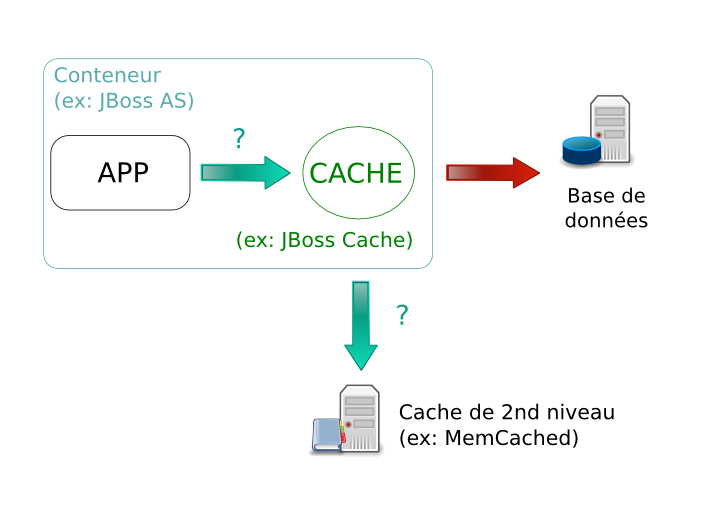
\includegraphics[scale=0.3]{img/cache-level.png}
      \caption{Niveau de cache (illustration)}
      \label{cache-level}
    \end{center}
  \end{figure}
}

\ifslide{
  \begin{frame}{Niveau de cache}
   \begin{center}
     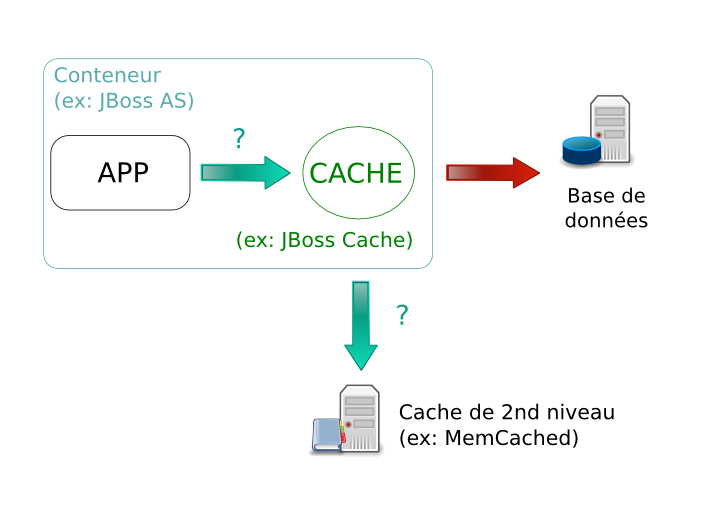
\includegraphics[scale=0.3]{img/cache-level.png}
   \end{center}
  \end{frame}
}

\ifbook {

  \mysubsubsection{Un exemple de stratégie de cache: le "long tail catalog"}

  \paragraph{} Pour illustrer notre propos sur l'importance des caches, étudions un cas classique
  des applications en ligne: le \textit{long tail catalog}. Ce scénario est simple, une boutique en
  ligne dispose d'un catalogue de taille N, où est N est beaucoup plus grand que la mémoire M,
  disponible pour l'application.

  \paragraph{} Compte tenu qu'il est relativement coûteux, en terme de performance, de retrouver les
  éléments du catalogue depuis la source de données, on optimise généralement le système en plaçant
  en cache, de taille N, les données les plus demandées.

  \paragraph{} Une implémentation simple, et élégante, consiste à placer toutes informations
  retrouvées depuis la source de données en cache, et lui associer une date de péremption (par
  exemple, une heure après sa mise en cache). À chaque fois que la donnée est retrouvé dans le
  cache, sa date de péremption est repoussée d'une heure.

  \paragraph{} Ainsi, après quelques heures d'exécutions, le cache de l'application contiendra les
  N données les plus souvent demandées du catalogue complet, contenant M élément. Il est donc
  vraisemblable que la plupart des requêtes effectuées par les clients de la boutique en ligne, soit
  assez rapide.

  \paragraph{} Les requêtes marginales seront bien évidemment moins performantes, mais l'impact
  négatif, en terme de vente, sera bien moindre...

  \begin{figure}[h]
    \begin{center}
      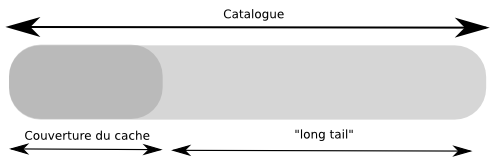
\includegraphics[scale=0.3]{img/long-tail-catalog.png}
      \caption{Le "Long tail catalog"}
      \label{cache-level}
    \end{center}
  \end{figure}
}

\ifslide{
  \begin{frame}{Le "Long tail catalog"}
   \begin{center}
     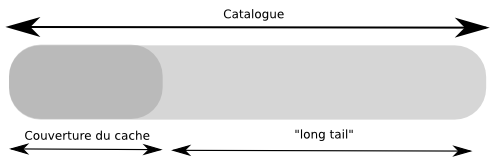
\includegraphics[scale=0.6]{img/long-tail-catalog.png}
   \end{center}
  \end{frame}
}

